\chapter{Device 1: prototype for spatio-angular illumination}
\begin{summary}
   - Im vorhergehende Kapitel haben wir das dem spatio-angularen
     Mikroskop zugrundliegende Konzept dargestellt. Hier gehen wir auf
     zusaetzliche Details ein, die fuer die praktische Implementierung
     wichtig sind. Unter anderem die Eigenschaften der beiden
     verwendeten Displays, elektronische Synchronisation der
     verschiedenen Komponenten und einem Algorithmus, um das
     Koordinatensystem der Kamerapixel und der Pixel des focal plane
     SLM ineinander zu transformieren.

   - Das pupil plane SLM wurde durch unseren Partner Fraunhofer IPMS
     waehrend des Projekts neu entwickelt.  Daher widmen wir uns diesem
     Subsystem im Kapitel (FIXME) naeher.
\end{summary}
\section{Description of the optical system with reflective displays}
 - Bisher haben wir den Strahlengang nur fuer Transmissionsdisplays
   gezeigt (in fig:memi-simple). Solche SLM haben in Praxis aber nur
   sehr geringe Transmission und deshalb verwenden wir in unserem
   System reflektive Displays. 

 - fig:memi-real zeigt schematisch den entsprechend angepassten
   Strahlengang.  Unten links strahlt die Lichtquelle in das
   System. Die Optik ist farbkorrigiert von 400 bis 700nm
   Wellenlaenge. Das System beleuchtet nacheinander den pupil plane
   SLM---den vom Fraunhofer entwickelten
   Graustufen-Mikrospiegelarray---und den focal plane SLM, ein
   kommerzielles liquid crystal on silicon Display.
  
 - Wenn wir einen Laser benutzen, dann senden wir den parallelen
   Strahl zunaechst durch ein Mikrolinsenarray. In der Fokusebene nach
   dem Array befindet sich hinter jeder Linse ein Spot. Das
   Mikrolinsenarray rotiert, so dass diese Spots waehrend einer
   Belichtungszeit der Kamera moeglichst viele Positionen abdecken.
   Durch diese Vorgehensweise koennen wir das Laserlicht, das generell
   hohe oertliche Kohaerenz---also eine geringe Etendue---aufweist, an
   die Etendue der nachfolgenden Optik anpassen. Mikrolinsen mit
   kuerzerer Fokuslaenge fuehren zu groesserer Etendue.

 - Durch mehrfache Reflexion in einem Lichttunnel\footnote{Der Tunnel
   hat einen quadratischen Querschnitt. priv. comm. mit Prof. Herbert
   Gross: "Wenn mit dem Querschnitt die Flaeche parkettiert werden
   kann, dann eignet sich der Tunnel zum Homogenisieren des Lichts".}
   erzeugen wir eine homogene Lichtverteilung in F'''. 
   
   (FIXME warum hat invision nicht zwei mikrolinsenarrays
   hintereinander gesetzt?, wieviel licht wird im tunnel absorbiert?)

 - Fuer Experimente mit einer LED Lichtquelle, haben wir diese immer
   in der Naehe von F''' platziert. Wir platzieren die Oberflaeche der
   LED absichtlich ausserhalb von F''', so dass ihre Details nicht im
   Sample sichtbar sind. LEDs sind Lambertstrahler und strahlen Licht
   in den vollen Halbraum. Eine Lichtemittierende Flaeche mit einigen
   10um reichen demnach aus um die Etendue von Mikroobjektiven zu
   fuellen. Die Auswahl brauchbarer LEDs ist schwierig, den die
   Datenblaetter enthalten selten Angaben ueber die strahlende
   Flaeche. Bei 3W LEDs haben wir einige mm gemessen. Fuer hoechste
   Intensitaet im Sample ist es daher besser, LEDs mit geringer
   Gesamtleistung und kleiner strahlender Flaeche zu verwenden. Diese
   lassen sich dann besser Kuehlen und bei hoeheren Strom betreiben.


\begin{figure}[!htbp]
  \centering
  \svginput{2}{memi-real}
  \caption{Schematic of the light path through our microscope. Laser
    light enters from the lower left, is scrambled and homogenized to
    illuminate the full MMA and LCoS. $F$ is the field plane in the
    sample and its primed versions are conjugated planes. $P$ is the
    pupil of the objective. $B_0$ and $B_1$ are adjustable circular
    apertures. PBS is a polarizing beam splitter. DBS is a dichromatic
    beam splitter.}
  \label{fig:memi-real}
\end{figure}

\jpginput{8cm}{integrator-rod}{integrator rod}



\jpginput{14cm}{setup-photo-blueprint}{The wide field epi-fluorescence
  microscope with attached illumination head. The positions of the two
  spatial light modulators (Micro mirror array (MMA) and liquid
  crystal on silicon display (LCoS)) are indicated. Drawing by Josef
  Wenisch (In-Vision, Austria).}

\jpginput{14cm}{memi-setup-only-lenses}{only lenses7}


\begin{figure}[!htbp]
   \centering
   \svginput{2}{memi-sketch}
   \caption{Schematic of the lenses in the MEMI system and their focal
     lengths. The focal length $f_\textrm{TL}$ of the tube lens can be
     varied. This allows to scale the second intermediate image
     $r''_\textrm{MMA}$ of the micro mirror array to fit the back
     focal plane of different objectives. Dimensions in mm.}
   \label{fig:memi-sketch}
 \end{figure}




% \imagw{14cm}{mma}{{\bf left:} Scanning electron microscope image of
%   the micro-mirror array (MMA).  The pixel pitch of the device is
%   \unit[0.016]{mm}. The hinges for the tilt movement and the
%   electrodes are clearly visible. {\bf middle:} Optical reflective
%   microscope image of the MMA. {\bf right:} exaggerated rendering of
%   how a 8x8 checker board pattern would be displayed on the
%   device. Electron and optical micrograph by Fraunhofer IPMS Dresden
%   (Germany)}

% \begin{figure}[!hbt]
%   \centering
%   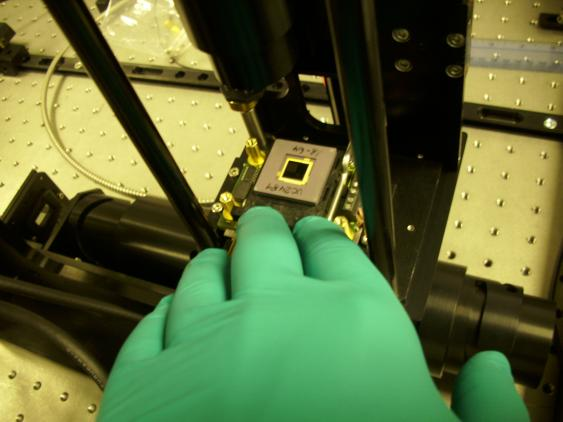
\includegraphics[width=7cm]{mma-plain}
%   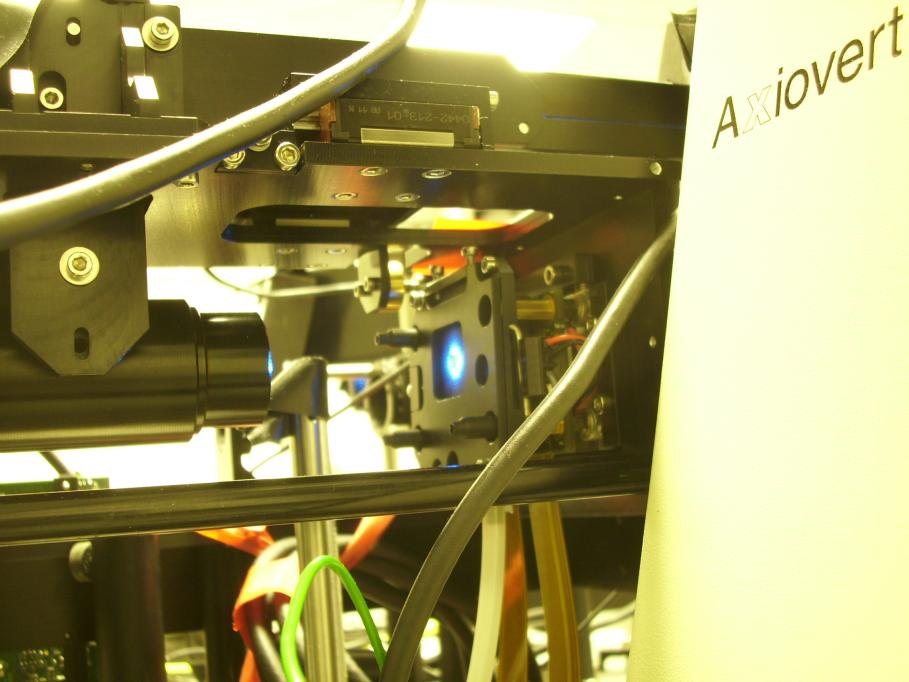
\includegraphics[width=7cm]{mma-ill}
%   \caption{{\bf left:} Micro mirror array chip during installation of
%     the optics. {\bf right:}~Illuminated micro mirror array in the
%     aligned system.}
%   \label{fig:mma-closeup}
% \end{figure}
